\documentclass{beamer}
\usetheme{simple}

\usepackage{amsmath}
\usepackage[export]{adjustbox}
\usepackage{graphicx}
\usepackage{lmodern}
\usepackage{transparent}
\usepackage[scale=2]{ccicons}

\setbeamercovered{invisible}

\title{Bayes Workshop 2}
\subtitle{Model Fitting and MCMC}
\date{\today}
\author{Corson N. Areshenkoff}
\institute{University of Victoria}

\begin{document}

\maketitle

\begin{frame}{The need for Bayesian models}
Setup:
	\begin{itemize}
		\item Police force in a city of 1,000,000 people with 100 criminals
		\item Lie detector with 99\% accuracy
		\item $H_0$: Person is innocent
	\end{itemize}
Experiment:
	\begin{itemize}
		\item Test one person and find guilty.
		\item p-value?
		\begin{itemize}
			\item 1\% false positive rate, so $p = 0.01$.
		\end{itemize}
		\item Probability that person is actually guilty?
		\begin{align*}
			P(H_1|D) &= \frac{P(D|H_1)P(H_1)}{P(D)} \\
					 &= \frac{0.99 \cdot 0.0001}
					   		 {0.99 \cdot 0.0001 + 0.01 \cdot 0.9999} \\
					 &\approx 0.001
		\end{align*}
	\end{itemize}
\end{frame}

\begin{frame}
    \begin{figure}
    \centering
        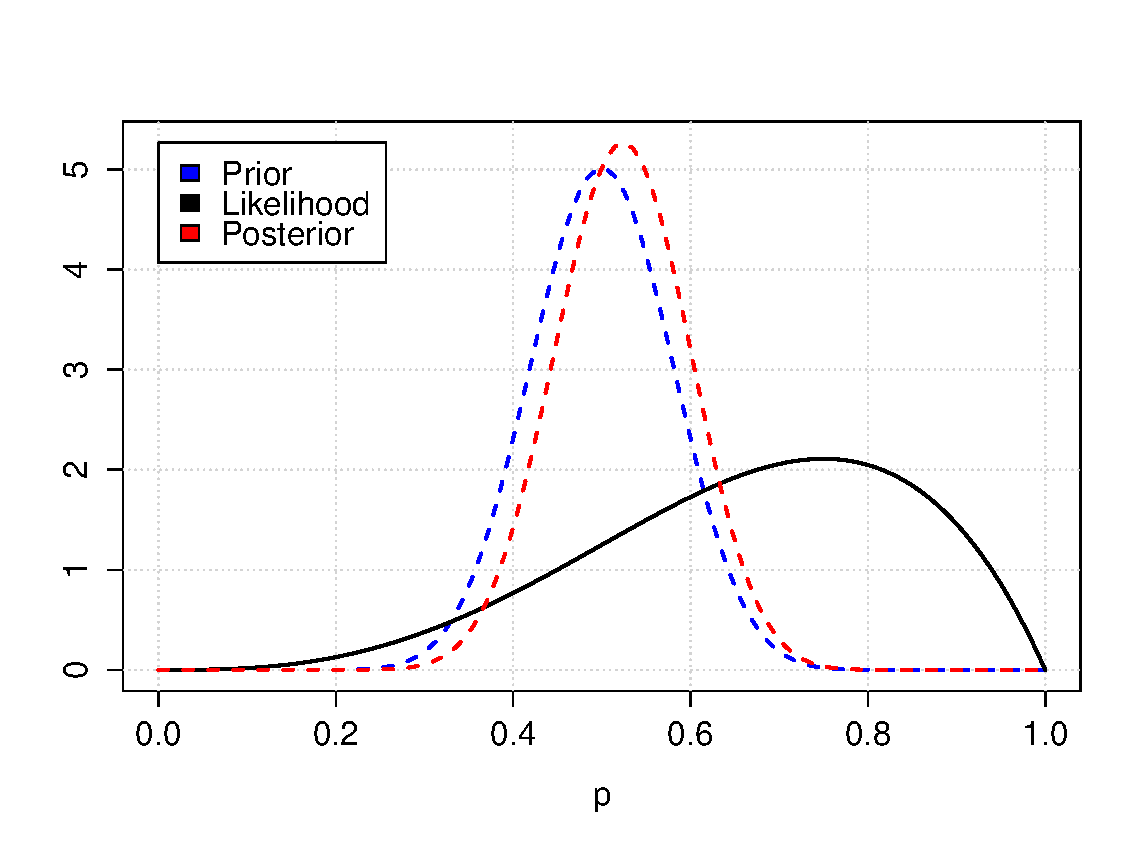
\includegraphics[width=.8\textwidth]{../images/binom_posterior.pdf}
        \caption{Binomial posterior for $N=4$ and $k=3$.}
    \end{figure}
\end{frame}

\begin{frame}{The Problem}
    \begin{itemize}
    \item Generally, we cannot compute the posterior distribution, so we have to approximate
          it numerically.
    \item How?
        \begin{itemize}
            \item Suppose we want to compute the mean $m$ of a normal distribution.
            \item Can compute it analytically:
                \[  m = \frac{1}{\sigma \sqrt{2\pi}} 
                    \int_{-\infty}^\infty xe^{\frac{(x - \mu)^2}{2\sigma^2}} \mathrm{d}x\]
            \item Or, can draw lots of samples from a normal distribution and compute the
                  empirical mean (numerical approach).
            \item Or, if we want to see the full distribution, we can plot a histogram of the 
                  samples.
        \end{itemize}
    \end{itemize}
\end{frame}

\begin{frame}[fragile]{The Problem}
    \begin{itemize}
        \item Another problem:
            \begin{itemize}
                \item If we want to draw samples from a normal distribution, we can use e.g.     
                      the \verb+rnorm()+ function in R.
                \item In general, there is no way to draw samples directly from a posterior
                      distribution.
            \end{itemize}
        \item The solution:
            \begin{itemize}
                \item Several algorithms (e.g. MCMC) can generate sequences of 
                      samples which converge in probability to the posterior distribution.
                \item i.e. The algorithm generates samples $(x_1,x_2,\dots,x_n,\dots)$, and 
                           the distribution of each observation gets closer to the posterior 
                           distribution as $n \rightarrow \infty$.
            \end{itemize}             
    \end{itemize}
\end{frame}

\begin{frame}{Working with MCMC}
General MCMC procedure:
    \begin{enumerate}
        \item Specify a model + prior.
        \item Use an MCMC "chain" to generate random samples from the posterior.
        \item How to tell if MCMC works?
    \end{enumerate}
\end{frame}

\begin{frame}{Working with MCMC}
    \begin{description}
        \item[Problem] Chains take a while to converge to the posterior distribution.
            \begin{description}
                \item[Solution] Let the chain "burn-in"; discard the first few samples.
            \end{description}
        \item[Problem] Hard to tell when convergence has taken place for a single chain.
            \begin{description}
                \item[Solution] Run multiple chains and verify that they generate similar 
                                samples.
                \item[Solution] Summary statistics (e.g. $\hat{R}$)
            \end{description}
        \item[Problem] Samples are not independent, so 100 samples from MCMC does "contain"
                       100 samples worth of information about the posterior.
            \begin{description}
                \item[Solution] Examine autocorrelation 
                \item[Solution] Effective sample size $n_\text{eff}$.
            \end{description}
    \end{description}
\end{frame}

\begin{frame}{Sample Model}
    \begin{itemize}
        \item Consider the problem of estimating a sample mean, where the sample is
              assumed to be normally distributed with known variance $\sigma^2 = 1$.
        \item We assume that the mean is close to zero, so we use a standard normal
              prior.
        \item Let $X = (x_1,x_2,\dots,x_N)$ be our sample. Then the model is written as
            \begin{align*}
                x &\sim \mathrm{N}(\mu, 1) \\
                \mu &\sim \mathrm{N}(0,1)
            \end{align*}
        \item In this case, we know that the posterior is
            \[ \mathrm{N} \left ( \frac{1}{N+1}\sum x_i, \frac{1}{N+1} \right ) \]
            so we can compare it with the results from MCMC.
    \end{itemize}
\end{frame}

\end{document}